% ON-THE-FLY
% explicar exploración parcial (lo visto hasta ahora)
% estados ganadores y perdedores ahora (antes era fácil, ahora tenemos que ver a dónde van)
% el concepto de ``frontera'' (en el sentido de transiciones existentes sin explorar) top, bottom
% actualizamos estado solo cuando estamos seguros (ganador en bottom / perdedor en top)
% exploramos de a una transición [e -l-> e']
% esto actualiza antecesores de e
% idea central de que ganador necesita loop


%dividimos en dos la explicación on-the-fly
%-------------------------------------------------------
\begin{frame}{Exploración parcial}
    La idea es intentar sacar conclusiones a medida que se explora, y construye a la vez, la composición total.
    
    Por ejemplo, en un momento dado podríamos tener explorado lo siguiente:
    \begin{figure}
     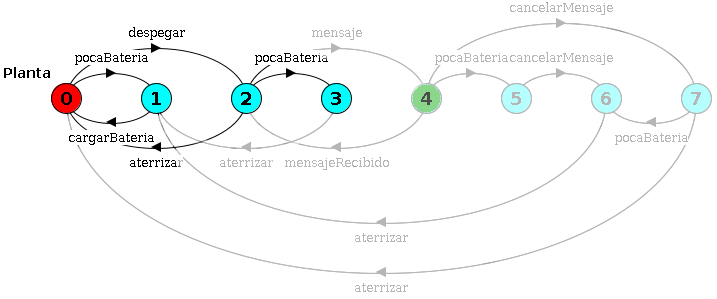
\includegraphics[width=\textwidth]{figures/partial.png}
    \end{figure}
    
    Exploramos de a una transición $e \step{\l}{} e'$ o paso.\vspace{10pt}\footnote{Los llamamos $e$ en vez de $t$ para resaltar que son \textit{estados de la planta}}
\end{frame}
%-------------------------------------------------------
\begin{frame}{Frontera optimista y pesimista}
    \begin{figure}
     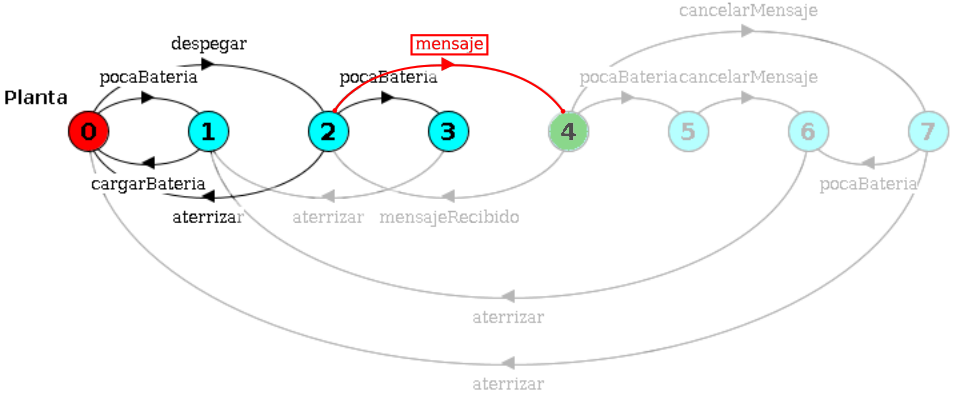
\includegraphics[width=\textwidth]{figures/frontera.png}
    \end{figure}
    El paso $2 \step{mensaje}{} 4$ está sin explorar. Como en principio no sabemos nada de él podríamos pensar que nos lleva a un estado ganador (frontera optimista) o perdedor (frontera pesimista).
\end{frame}
%-------------------------------------------------------
\begin{frame}{Nueva definición de ganadores/perdedores}
    Antes era simple reconocer ganadores/perdedores porque contábamos con toda la información de la planta; ahora debemos ``imaginar'' a dónde van a parar las transiciones no vistas.
    
    Actualizamos estados sólo cuando estamos seguros, es decir, señalamos ganadores sólo al pensar una frontera pesimista y perdedores en el caso contrario.
    
    \begin{block}{Observación}
        Los estados ganadores/perdedores según esta definición son ganadores/perdedores en la planta completa, es decir, una vez que clasificamos un estado nunca debemos reconsiderarlo.
    \end{block}
\end{frame}
%------------------------------------------------------- %parte 2
\begin{frame}{Propagar información}
    Lema2 ganador/perdedor es antecesor explicar por qué o lema o ej de imágen, ver la mejor manera\\
    Lema3 hay info para propagar si e' era conocido Y era gandor/perdedor (cc. no sabemos nada nuevo)
\end{frame}
%-------------------------------------------------------
\begin{frame}{Obtener nueva información (Ganador)}
    Lema4 como dijimos antes, necesitamos un loop para ganar, entonces sólo va a haber ganadores nuevos al encontrarnos dicho loop (i.e. el e' es uno que vimos Y no es ni ganador/perdedor porque sino cae en el caso anterior)
\end{frame}
%-------------------------------------------------------
\begin{frame}{Obtener nueva información (Perdedor)}
    Lema5 si ya exploraste todo y no hay marcados por ningún lado entonces obvio que no podés llegar a ninguno [dibujo]
\end{frame}
%-------------------------------------------------------
\begin{frame}{Resúmen del nuevo algoritmo}
    \begin{itemize}
     \item Clasificamos (ganador/perdedor) cuando estamos seguros. %i.e. no se cambia una vez que está
     \item Propagamos a los antecesores afectados (si hay información respecto a e').
     \item Tratamos de obtener nueva información sólo al cerrar loops.
    \end{itemize}
    
    \begin{block}{Observación:}
        Sólo hacemos nuevos cálculos cuando son realmente necesarios.
    \end{block}
    
    Nos interesa saber qué tan buena es la eficiencia del algoritmo, en tiempo de cómputo.
\end{frame}


